\documentclass[../report.tex]{subfiles}

\begin{document}
\subsection{Đề bài} \cite{problem-993e}
\begin{figure}[H]
\centering
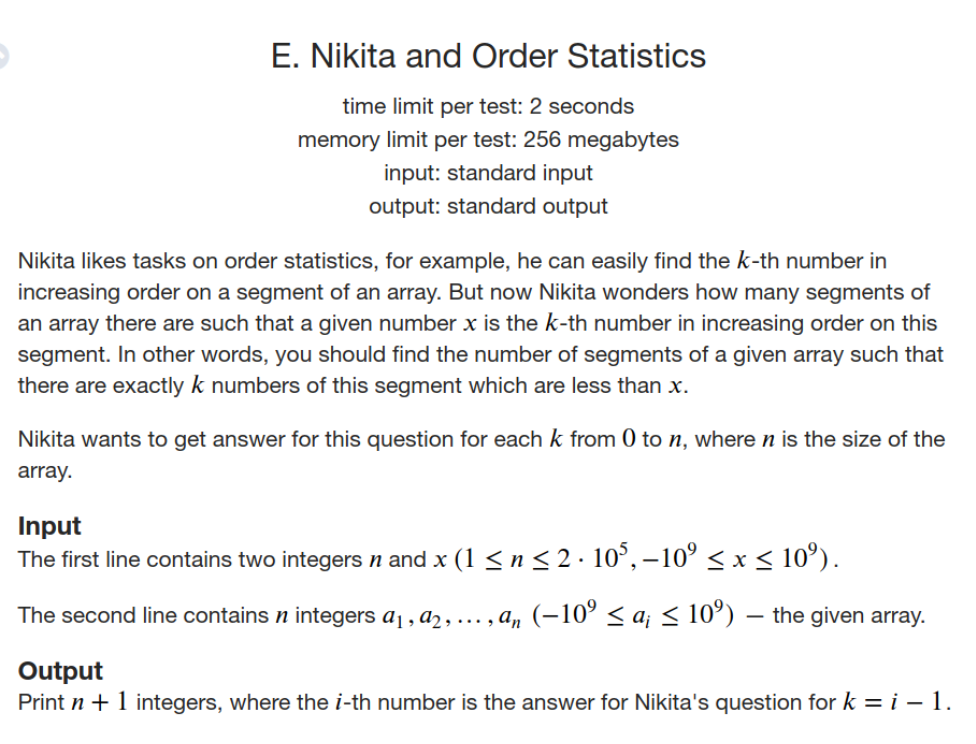
\includegraphics[width=\textwidth]{figures/993E.png}
\end{figure}

\subsection{Tóm tắt}
Cho một mảng n phần tử và một giá trị x. \\
Ứng với mỗi giá trị k từ 0 đến n, tìm số lượng các đoạn (segment) 
mà có đúng k giá trị trong đoạn đó là nhỏ hơn x.  \\
Điều kiện:
\begin{align*}
    1 &\le n \le 2 \times 10^5 \\
    -10^9 &\le a_i \le 10^9 \\
    -10^9 &\le x \le 10^9
\end{align*} \\
Giới hạn thời gian: 2s, bộ nhớ: 256MB. 

\subsection{Ý tưởng lời giải}
Ý tưởng lời giải: 
\begin{itemize}
    \item Do ta chỉ quan tâm các vị trí trong mảng có nhỏ hơn x 
        hay không, nên ta có thể chuyển 
        mảng đầu vào thành chuỗi nhị phân. 
        Ví dụ với $x = 3$:
    \begin{figure}[H]
    \centering
    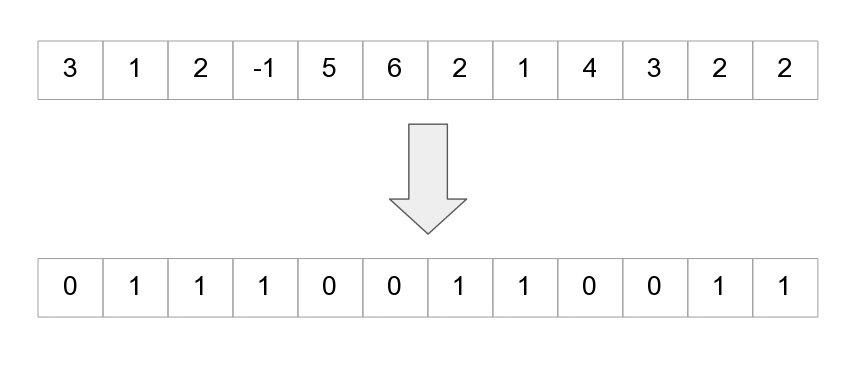
\includegraphics[width=10cm]{figures/convert-to-binary.png}
    \end{figure}

\item Gọi $C_j$ là số các số 0 sau phần từ 1 thứ j, cộng 1. 
    ($j = \overline{1, m}$) và $C_0$ là số 
    phần tử 0 liên tiếp bắt đầu xâu nhị phân M, cộng 1. 
    \begin{figure}[H]
    \centering
    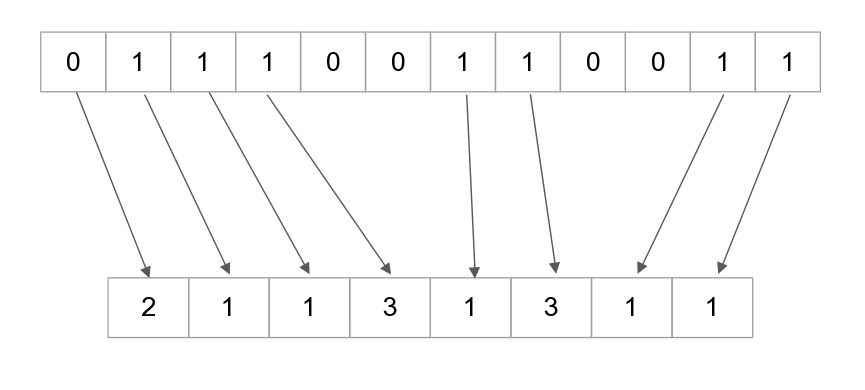
\includegraphics[width=10cm]{figures/C_j.png}
    \end{figure}

\item Số các segment gồm k ($k \ge 1$) số 1 bao lấy đoạn ứng với $C_j$ đến 
    $C_{j + k - 1}$ là: 
\begin{align*}
    X_k &= \sum_{j = 1}^{m + 1 - k} C_{j - 1} \times C_{j - 1 + k}  \\
    &= \sum_{p = 0}^{m - k} C_{p} \times C_{p + k} 
\end{align*}\\

\item Ta chuyển công thứ trên thành nhân đa thức: \\
Gọi $D$ là dãy nghịch đảo của $C$. \\
Hay: $D_i = C_{m - i} \quad\forall i = \overline{0, m}$ \\
Ta có:
\begin{align*}
    C_{p + k} &= D_{m - k - p} \\
    \Rightarrow X_k &= \sum_{p = 0}^{m - k} C_{p} \times C_{p + k}\\
    &= \sum_{p = 0}^{m - k} C_{p} \times D_{m - k - p}\\
\end{align*}\\
Công thức này chính là công thức nhân đa thức, từ đó ta có thể 
sử dụng FFT để tính nhanh các giá trị $X_k$. 
\end{itemize}

\subsection{Code của thuật toán}
\begin{lstlisting}
void init() {
    std::fill(C, C + n + 1, 0);
    C[0] = 1;

    C_len = n + 1;
    bit_count = ceil_log2(C_len * 2);
    N = 1 << bit_count;

    init_T(bit_count);
}

void input() {
    std::cin >> n >> x;

    init();

    ll sum = 0;
    for (ll i = 0; i < n; i++) {
        ll v;
        std::cin >> v;
        sum += v < x;
        C[sum]++;
    }

    for (ll i = 0; i <= sum; i++)
        if (C[i] > 1) 
            zero_count += C[i] * (C[i] - 1) / 2;
}

int main() {
    std::ios::sync_with_stdio(false);

    input();
    std::cout << zero_count << " ";
    static cp A[FFT_MAX], B[FFT_MAX];

    std::copy(C, C + C_len, A);
    std::fill(A + C_len, A + N, 0);

    std::fill(B, B + 2 * n - C_len, 0);
    std::reverse_copy(C, C + C_len, B + 2 * n - C_len);
    std::fill(B + 2 * n, B + N, 0);

    fft(A, bit_count);
    fft(B, bit_count);
    for (ll i = 0; i < N; i++)
        A[i] *= B[i];
    fft(A, bit_count, true);
    for (ll k = 1; k <= n; k++)
        std::cout << (ll)std::round(A[2 * n - k - 1].real()) << " ";
    std::cout << '\n';
    return 0;
}
\end{lstlisting}
Trong đó init\_T là hàm để khởi tạo bảng chuyển vị bit. 
($T[i]$ sẽ là số tương ứng với các bit đảo ngược của i). 
Hàm input sẽ thực hiện đọc đầu vào và chuyển luôn thành mảng 
$C_i$, không thông qua bước chuyển thành chuỗi nhị phân. Thời gian 
tính toán $\mathcal{O}(n)$.

Thực  hiện sao chép giá trị của C cho vào mảng A,
đảo ngược giá trị của mảng C, cho vào 
mảng B. Thực hiện nhân nhanh đa thức bằng FFT và in kết quả. 

Giá trị zero\_count là số các đoạn mà không chứa số 1 nào phải được 
tính riêng lẻ. 

\subsection{Bộ test và kết quả chạy} 
Bộ test chương trình: 
\begin{itemize}
    \item 6 test tay (kết quả được tính bằng tay), bao gồm một 
        số test trên Codeforces. 
    \item 2 test có quy luật (đều nhỏ hơn x và đều lớn hơn x), 
        kích thước 20000 phần tử. 
    \item 2 test có quy luật (đều nhỏ hơn x và đều lớn hơn x), 
        kích thước 200000 phần tử. 
    \item 10 test được sinh ngẫu nhiên bằng chương trình đơn giản 
        (không dùng FFT) để kiểm tra tính đúng đắn, kích thước 
        20000 phần tử. 
    \item 10 test được sinh ngẫu nhiên bằng 
        chương trình đích để kiểm tra thời gian chạy, 
        kích thước 200000 phần tử. 
\end{itemize}
Kết quả chạy test: 
\begin{figure}[H]
\centering
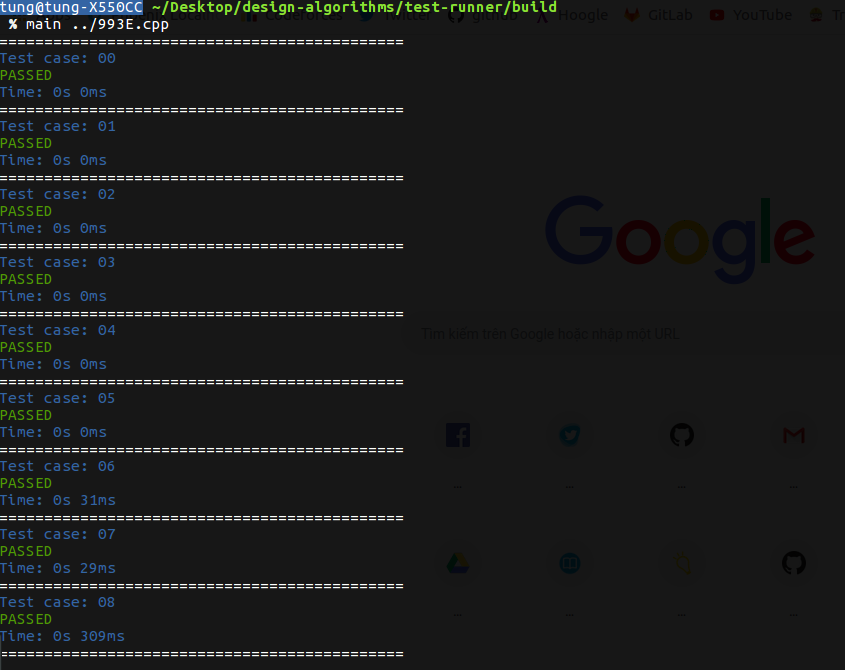
\includegraphics[width=\textwidth]{figures/test-993e-1.png}
\end{figure}

\begin{figure}[H]
\centering
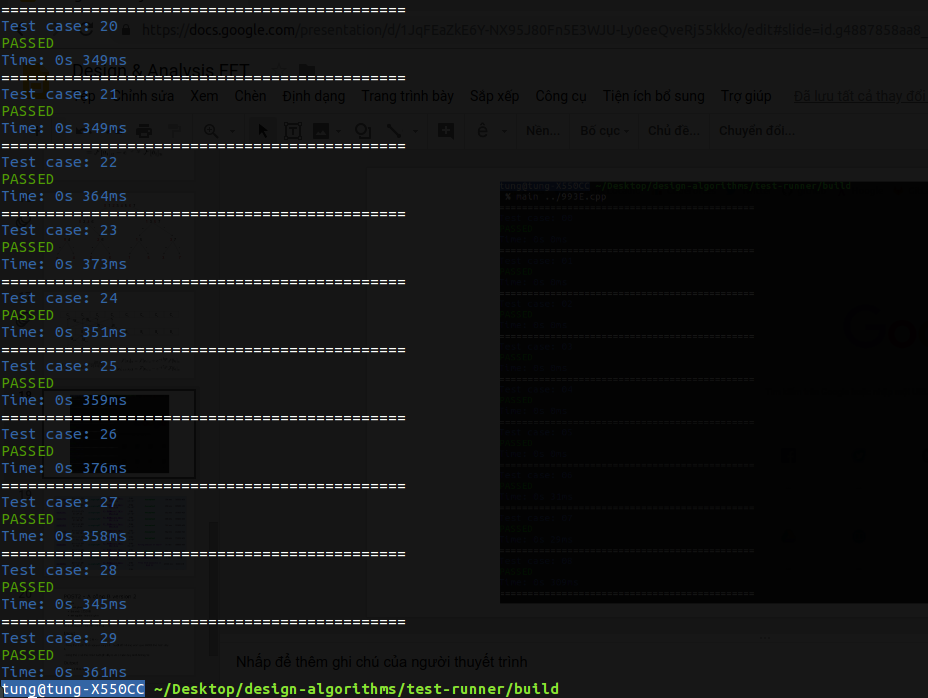
\includegraphics[width=\textwidth]{figures/test-993e-2.png}
\end{figure}

\subsection{Kết quả submit online}
\begin{figure}[H]
\centering
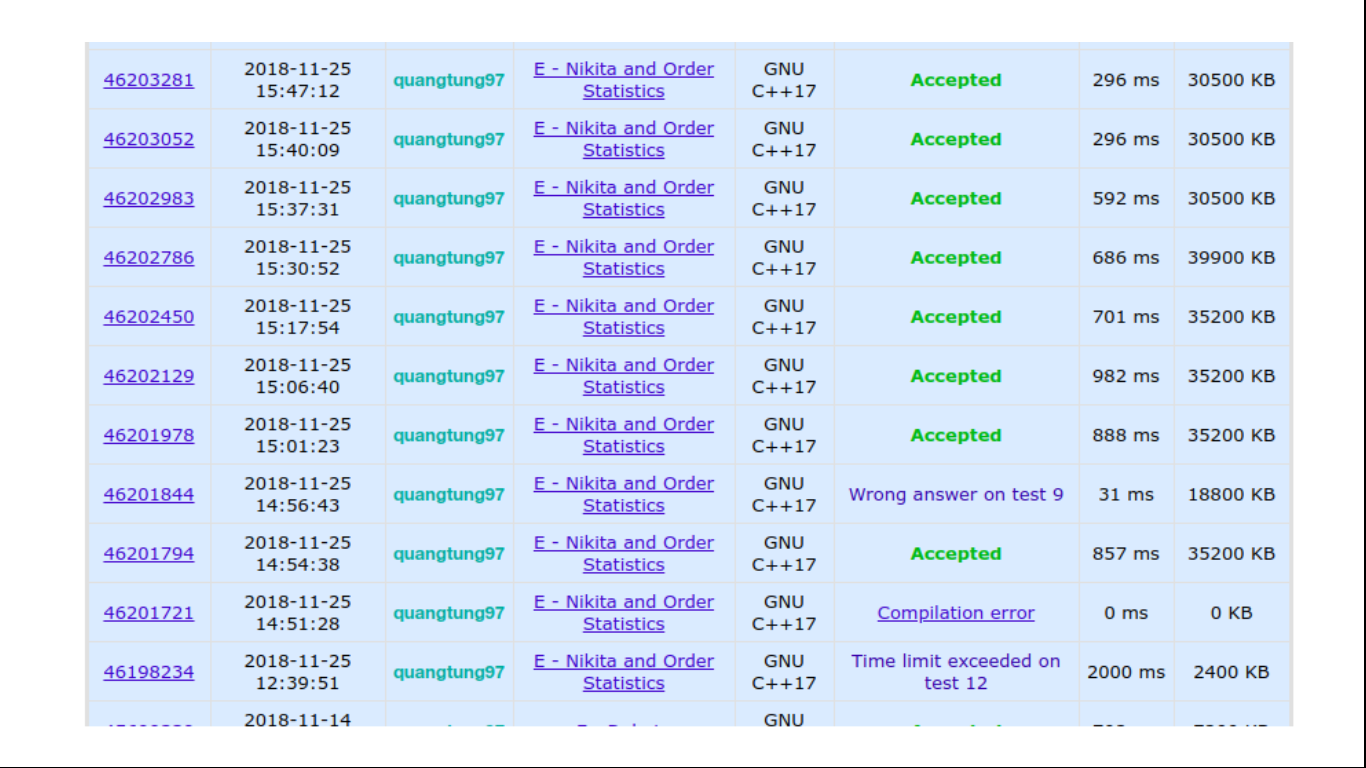
\includegraphics[width=\textwidth]{figures/submit-993e.png}
\end{figure}
\end{document}
